\documentclass[]{template/llncs}
\usepackage{url}
\usepackage{graphicx}
\usepackage{amsmath}
\usepackage{amsfonts}
\usepackage[linesnumbered,ruled,vlined]{algorithm2e}
\usepackage[
colorlinks = true,
linkcolor = black,
anchorcolor = black,
citecolor = black,
filecolor = black,
urlcolor = black
]{hyperref}
\usepackage{xeCJK} 
\setCJKmainfont{PingFangSC-Light}

\begin{document}
\bibliographystyle{unsrt}
\pagestyle{plain}

%
\title{ZKSwap: a Layer-2 Token Swap Protocol based on ZK-Rollup}

\author{L2 Lab}

\institute{
\email{dev@l2lab.org} \\
\vspace{0.5cm}
\today
}

\maketitle

%
\section{Introduction}

Since 2019, the blockchain industry has undergone breathtaking changes. Decentralized finance -- DeFi -- continues to grow at an exponential rate. The Total Value Locked in different DeFi protocols has exceeded 10 billion U.S. dollars. With the continuous development of numerous on-chain assets and off-chain assets going on-chain, we believe that the Total Value Locked in DeFi protocols will soon exceed 100 billion U.S. dollars. These on-chain assets require fast, frictionless, trust-free, and real-time exchange services, which has led to the rise of new decentralized exchange(DEX) protocols such as Uniswap\cite{uniswapofficial}.

Although the new DEX model spearheaded by Uniswap has achieved significant development, it still has obvious drawbacks. First, the high gas fee of dozens of dollars per transaction hinders new users to entry; second, every transaction and every execution needs to wait for at least one block to confirm, which gives an unsatisfactory experience; and third, subject to the limiting TPS of Ethereum, Uniswap has a clear bottleneck in transaction numbers and transaction capacity per second. Those drawbacks are not unique on Uniswap. They are common issues faced by all DEXes.

ZK-Rollup\cite{zkrollups} is a new type of Layer-2 scalability solution. Compared with other Layer-2 scalability solutions such as Plasma, ZK-Rollup has considerable advantages in terms of security, cost, TPS, and usability. It is especially suitable for building a Layer-2 decentralized exchange.

ZKSwap (a ZK-Rollups based Swap protocol) is a brand-new exchange protocol based on ZK-Rollups technology. Through Zk-Rollups technology, all ERC20 tokens are transferred to Layer2, and the consistent state of Layer1 and Layer2 is guaranteed based on continuously generated zero-knowledge proofs. This solution allows all exchanges to execute on Layer 2, achieving real-time swap with zero gas fees, unlimited scalability, removing the constraint from the Ethereum's TPS, and block confirmation time. The user no longer has to wait for the one-block confirmation time for each transaction. ZKSwap enables a DEX to provide the smooth user experience of a centralized exchange(CEX) while allowing the users to have full custody over their funds. We believe that ZKSwap is the future form of trading. It will trigger a significant evolution of all existing DEX and CEX.

At present, the ZKSwap team has finished most of the development work. We will release the ZKSwap exchange protocol in early October. In the future, we will promote the DEX exchange standard on Layer-2, so that all existing DEXes can seamlessly access and use the ZKSwap exchange protocol.


\section{Technical Overview
}

\subsection{Uniswap V1}
Uniswap\cite{uniswapv1} is an automated liquidity protocol powered by a constant product formula and implemented in a system of non-upgradeable smart contracts on the Ethereum blockchain. Users can create a liquidity pool by providing a certain percentage of ETH and any other ERC20 asset. One liquidity pool reserves ERC20 tokens and provides liquidity for the transactions between these two assets. In return, all liquidity providers will split the 0.3\% of the transaction volume as a liquidity provider fee. In Uniswap, the first liquidity provider needs to set the ratio of the two assets in the liquidity pool. The automated market maker algorithm will ensure that the product of the two assets before and after each transaction remains constant. The following is a brief introduction to the basic key concepts of Uniswap to help users understand related concepts coming up next.


\subsubsection{Create a Liquidity Pool}

In Uniswap, each trading pair has only one liquidity pool, which is generally created by the first liquidity provider. For example, a liquidity provider creates an ETH-ZKS liquidity pool, and then adds liquidity. The initial amount of ETH deposited is $x_0$, the number of ZKS stored is $y_0$, and $x_0*y_0 = c_0$. Here ZKS can be any ERC-20 token.


\subsubsection{Liquidity Token}

Liquidity Provider (hereinafter referred to as LP) will obtain the Liquidity Provider Token, (hereinafter referred to as LP Token or LT), which is used to represent the share of LP in the current liquidity pool. LP Token is an ERC-20 token that can be transferred without removing the liquidity of the liquidity pool. Each liquidity pool has a corresponding LP Token. 

The above-mentioned initial LP will receive $n_0 = \sqrt {x_0 * y_0} - MIN\_LIQUIDITY$ number of LP Tokens. Among them, since the total amount of LP Token will be used as the denominator in subsequent calculations, when adding liquidity for the first time, the system will set $MIN\_LIQUIDITY$, as the minimum reserved amount of LP Token, send it to address 0x0 to prevent the total amount of LP Token from becoming zero.

The following assumes that at any time $i$, there are $x_i$ ETH and $y_i$ ZKS in the liquidity pool, their product constant is $c_i = x_i * y_i$, and the total amount of LT issued is $n_i$. Among them, $i = 0, 1, 2, …$

\subsubsection{Create Liquidity}

When adding liquidity to an existing pool, users must deposit pair tokens proportional to the current ratio. Suppose a new LP deposits $X$ ETH and $Y$ ZKS to the liquidity pool, the LP must ensure that $X/Y = x_i/y_i$. The LP will in turn receive the newly minted $N = n_i*X/x_i$ number of LP Tokens. After adding liquidity, the reserve of the liquidity pool will be $x_{i+1}*y_{i+1} = (x_i+X)*(y_i+Y) = c_{i+1}$. The total amount of LP Token is $n_{i+1} = n_i + N$.


\subsubsection{Remove Liquidity}

LP can remove liquidity by burning their LT in the liquidity pool contract to withdraw their share of ETH and ZKS tokens from the pool. Assuming that the amount of LT burned by LP is $N'$, the amount of ETH that LP can withdraw is $X'= x_i*N'/n_i$, and the amount of ZKS tokens is $Y'= y_i*N'/n_i$. After the liquidity is removed, the reserve of the liquidity pool will be updated to $x_{i+1}*y_{i+1} = (x_i-X')*(y_i-Y') = c_{i+1}$. The total LT is updated to $n_{i+1} = n_i-N'$. Please note that the reserves of the liquidity pool might be different at the time when the LP deposits and when they withdraw, therefore the number and the ratio of tokens the LP can withdraw might change accordingly.  


\subsubsection{Swap Transaction}

After the liquidity pool is created and liquidity is injected, users who hold ETH or ZKS can start swapping in the liquidity pool. Here we use exchanging ETH for ZKS as an example. The user transfers m ETH to the liquidity pool, and the ETH in the liquidity pool will become $x_{i+1} = x_i + m$, and the user, in turn, receives $y_{i+1}$ ZKS tokens. According to the AMM algorithm in Uniswap, after deducting the $0.003*m$ fee, the remaining ZKS token amount should be $(x_{i+1} - 0.003m)*y_{i+1} = x_i*y_i$. Therefore, the user will get $y_{i+1} = (x_i*y_i)/(x_{i+1} - 0.003m)$ ZKS tokens. The liquidity provider fee will be automatically added to the liquidity pool after the transaction reserve, so after the transaction, the reserve of the entire liquidity pool becomes $x_{i+1}*y_{i+1} = c_{i+1}> c_i$. Since there is no other LP Token minted or burned at the moment, the total amount of LP Token remains unchanged, that is, $n_{i+1} = n_i$. This means that the ratios of all LPs remain the same, but each unit share now corresponds to more amount of the liquidity pool reserve.



\subsection{Uniswap V2}
Uniswap V1 implements basic AMM exchange functions, but there were also some issues. Since its contract is not upgradeable, in order to fix this problem, the development team re-implemented Uniswap V2 \cite{uniswapv2}, with basic functions the same as Uniswap v1 and some new features including


\begin{itemize}
	\item The users can directly create a trading pair of two ERC-20 tokens, instead of using ETH as an intermediary in Uniswap V1;
	\item A more reasonable price oracle, using the randomness of the price of the transaction before the first transaction in the block to make the price hard to manipulate; 
	\item Flash Swap, where users can obtain the target token first, and complete the swap later; or they can return the tokens within a certain time, so as not to trigger the swap process, which is equivalent to borrowing tokens in the liquidity pool;
	\item The original 0.3\% liquidity provider fee can be divided into two parts, of which 0.25\% is still used to split by liquidity providers proportional to their contribution to liquidity reserves, and 0.05\% is sent to the pre-set address as the Protocol Fee, which can be used for different purposes;

\end{itemize}

These new features increase the usability of Uniswap. For the exchange functionality, ZKSwap remains the same as Uniswap V2.

\subsection{ZK-Rollup and zkSync}
ZK-Rollups is a popular Layer 2 scalability solution. Its basic idea is to aggregate a large number of transactions then verify the proof on-chain. ZK-Rollups analyzes and verifies these aggregated transactions through smart contracts, and uses zero-knowledge proof technology to put the proof of aggregate transactions on-chain, thereby reducing the data that needs to be stored on-chain. All funds are locked in the smart contract, and most of the calculations and storage are done off-chain.

zkSync\cite{zksync} is one implementation of ZK-Rollups, and its v1 version is currently deployed on the Ethereum mainnet. Its basic working principle is as follows:

\begin{itemize}
	\item The user submits the signed transaction to the Validator;
	\item The Validator rolls up multiple transactions they have received within a period of time, merges them into one block, updates the root hash of the contract state tree, and sends the SNARK proof corresponding to the state update to the contract on-chain. This SNARK proof can prove that the new state is indeed the series of trading results modified to the old state;
	\item In addition, the Validator will also send the state delta ∆ corresponding to each transaction on-chain, which allows anyone to reconstruct the state after each transaction;
	\item The above SNARK proof and the delta ∆ of the blockchain state both need to be verified by the on-chain contract to prove the validity of all transactions and the data availability; 
\end{itemize}

Since the gas for SNARK proof is much less than the sum of gas to verify a large number of individual transactions and storing the full state off-chain is also much cheaper than storing it on-chain. Therefore, ZK-Rollup can theoretically achieve 100~200 times more scalability than the Ethereum mainnet while significantly reducing gas consumption.

The security of ZK-Rollup is almost the same as that of the corresponding Layer 1, because:


\begin{itemize}
	\item The Validator cannot tamper with the state, nor can it embezzle any Layer 2 funds, because all state changes need corresponding proof, which cannot be forged; and the private key is always in the hands of the user.
	\item Since the delta ∆ of the blockchain state and related proofs are stored on-chain, even if the Validator stops working, users can restore every transaction and retrieve the locked Token from on-chain data;
	\item The user does not need to stay online because there is no need to store any additional data.
\end{itemize}

zkSync currently supports three operations:

\begin{itemize}
	\item Deposit: transfer Tokens on Layer 1 to zkSync Layer 2;
	\item Withdraw: withdraw Tokens from the account on Layer 2 and send it to the account on Layer 1;
	\item Transfer: transfer Tokens on Layer 2 without the need for gas fees.
\end{itemize}

\section{ZKSwap Decentralized Swap Protocol}

This white paper implements a Layer 2 AMM decentralized transaction protocol ZKSwap. Based on ZK-Rollup technology, ZKSwap executes the full functionality of Uniswap on Layer 2, while ensuring the core value of decentralized exchange, ZKSwap increases the TPS by multiple orders of magnitude compared to Uniswap, and transaction processing hardly consumes any gas fees.

\subsection{ZKSwap System Architecture}

The ZKSwap system consists of on-chain smart contracts, off-chain ZKSwap Server, the zero-knowledge proof system, and front-end user interface.

\begin{figure}[htbp]
\centering
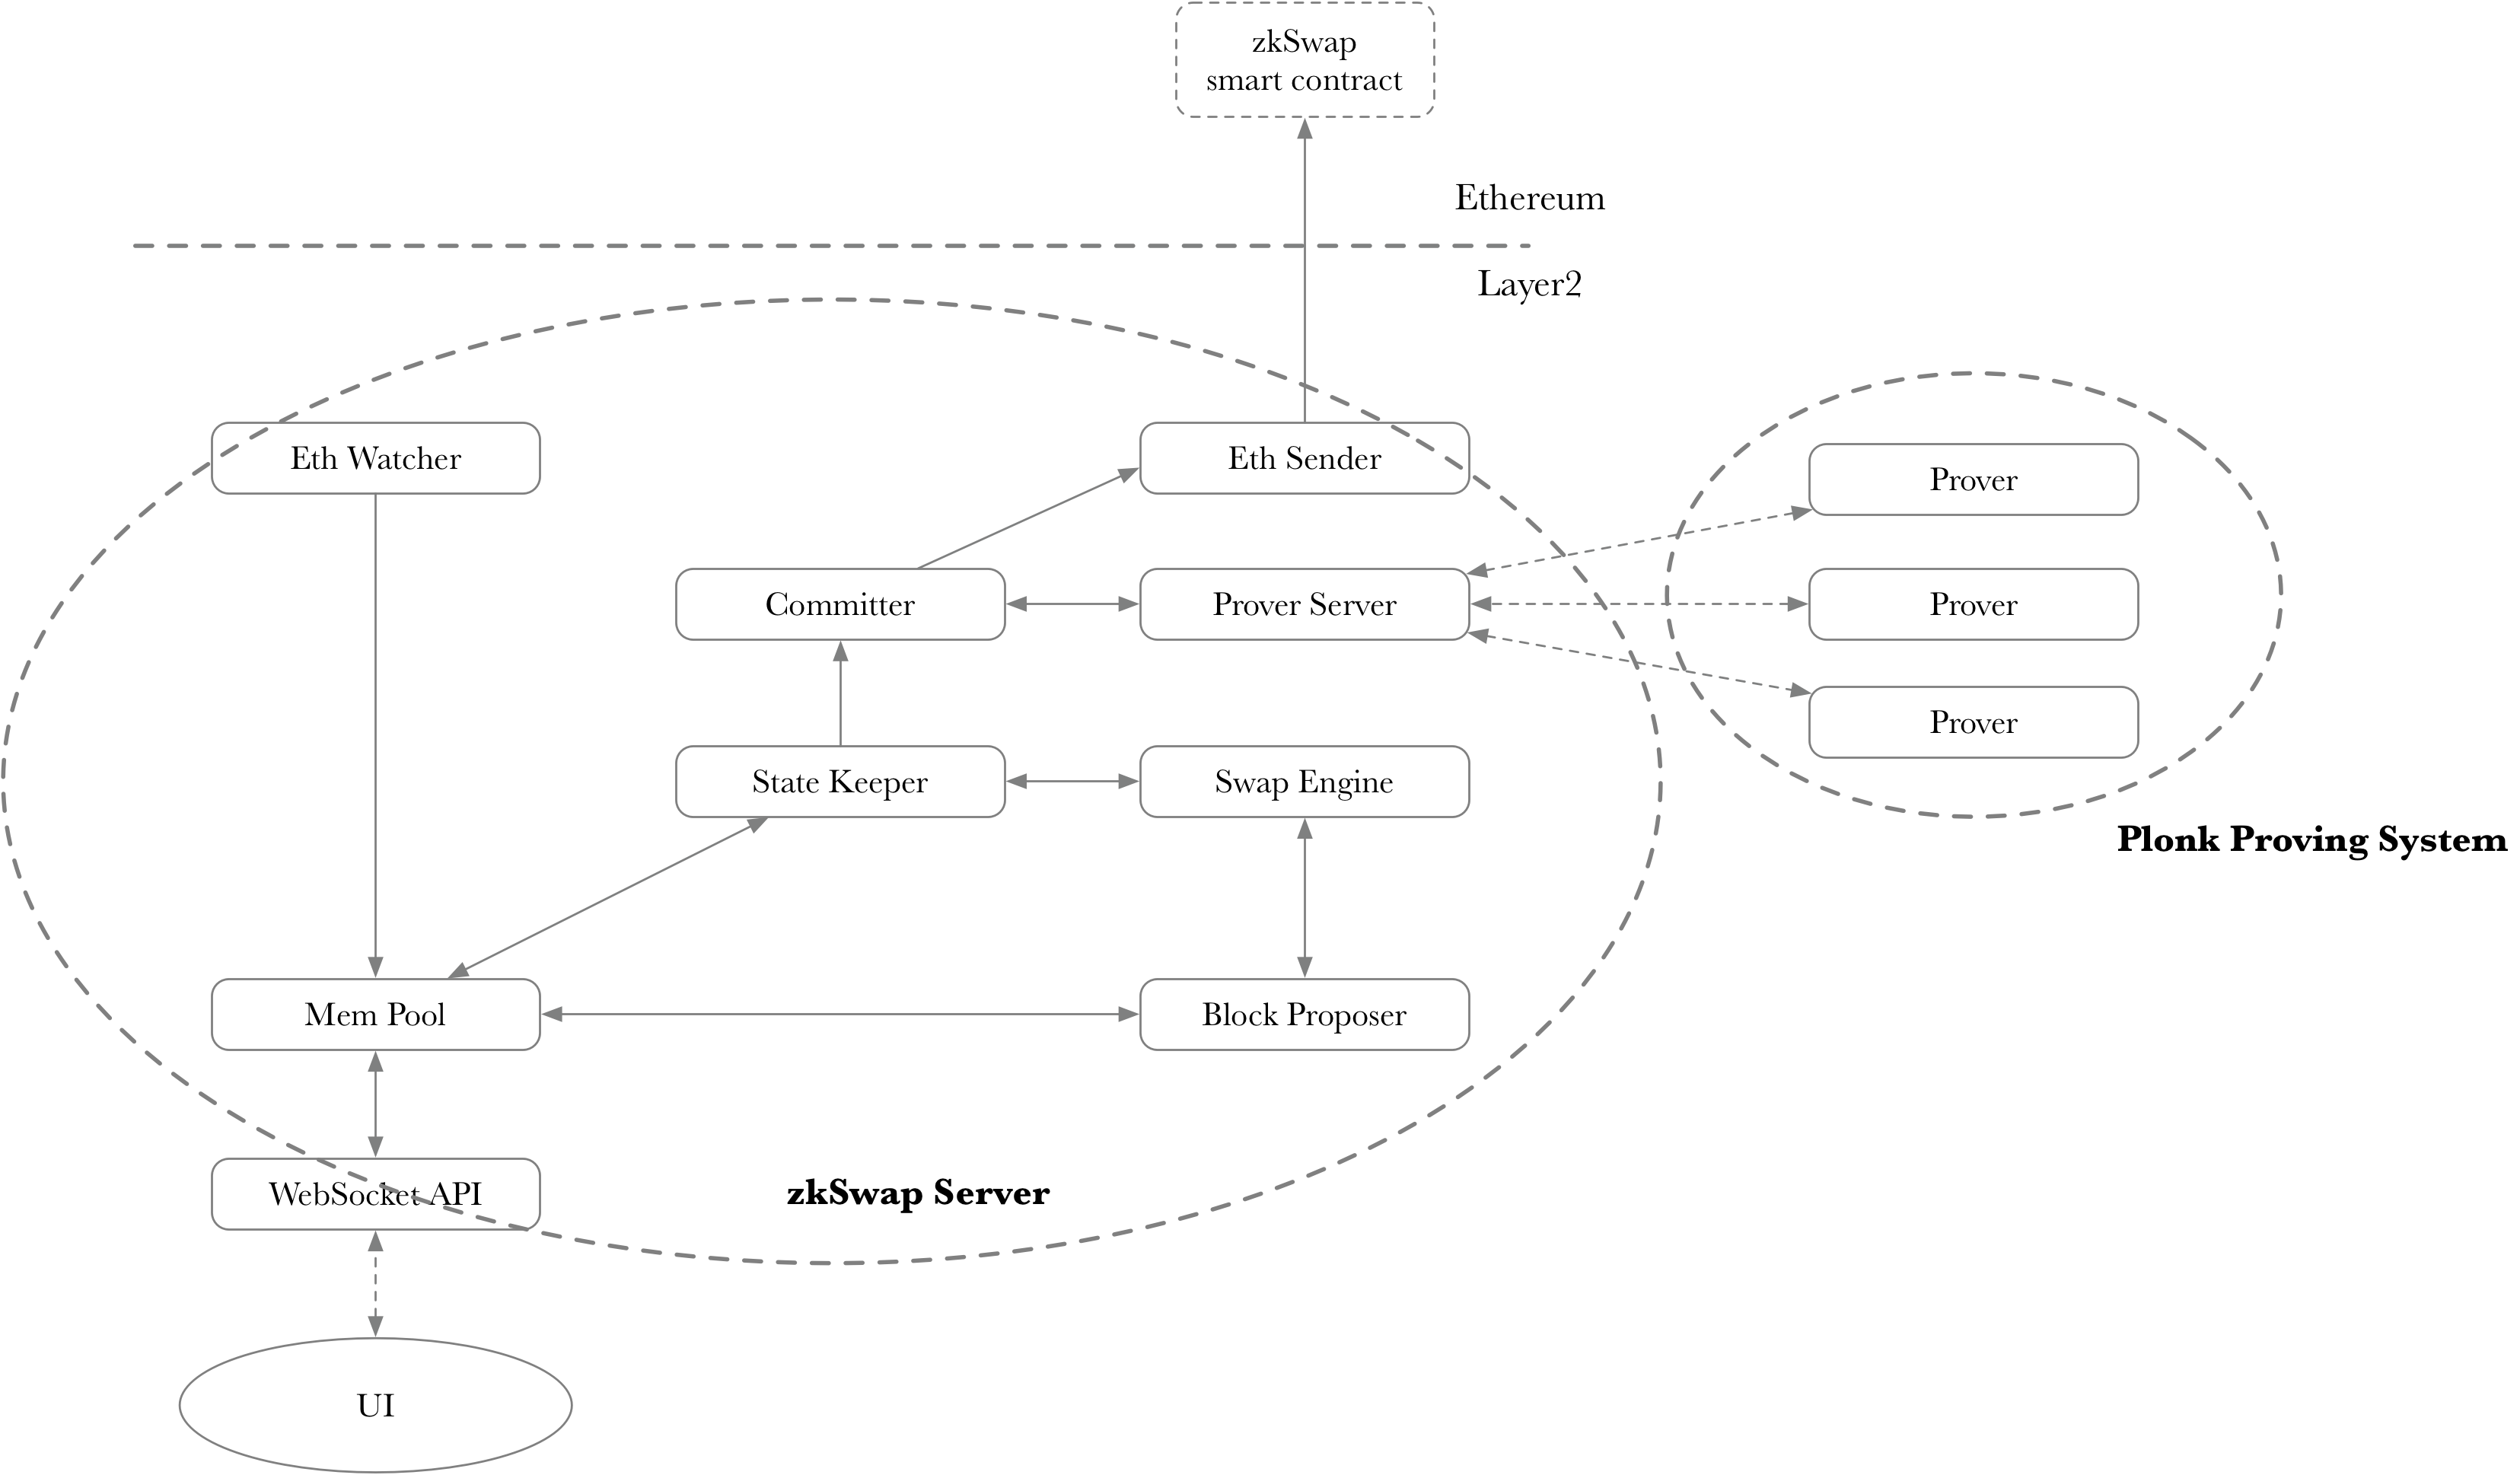
\includegraphics[width=0.9\columnwidth]{figure/arch}
\caption{System architecture}
\label{fig:arch}
\end{figure}

\subsubsection{ZKSwap Smart Contract}

ZKSwap will deploy a series of smart contracts on the Ethereum blockchain to store the tokens deposited by users while recording and verifying Layer 2 status updates and related proof. Those smart contracts are the key hub connecting on-chain and off-chain.


\subsubsection{ZKSwap Layer 2 Server}

The ZKSwap server is the module that processes all transactions off-chain. The ZKSwap server can use the WebSocket to interact with the user, and monitor transactions on the Ethereum blockchain. All valid transaction requests will be put into the ZKSwap mem pool and processed by the Swap Engine. The transaction types in the mem pool are the same as the transaction types of Uniswap. 
The Block Proposer will roll up the transactions and generate a new block. The State Keeper will update the status of all tokens on Layer 2. The State Keeper will send the state to the Commiter, which is responsible for communicating with the Prove Server, obtain the proof of the corresponding transaction, and finally send the state and the corresponding SNARK proof via Ethereum sender to the ZKSwap smart contract on-chain.


\subsubsection{Plonk Zero-knowledge Proof System}

ZKSwap's zero-knowledge proof system adopts a distributed architecture and uses the latest zero-knowledge proof algorithm PLONK\cite{cryptoeprint:2019:953} to generate proofs. The Prove Server supports multiple Provers. Multiple Provers actively query the proof tasks in the Prove Server and send them back to the Prover Server after generating the proof. PLONK's global trust setup only needs to be generated once, and the circuit can be greatly reused within a certain range, reducing the threshold for using zero-knowledge proofs.

\subsection{ZKSwap state tree}

\begin{figure}[htbp]
\centering
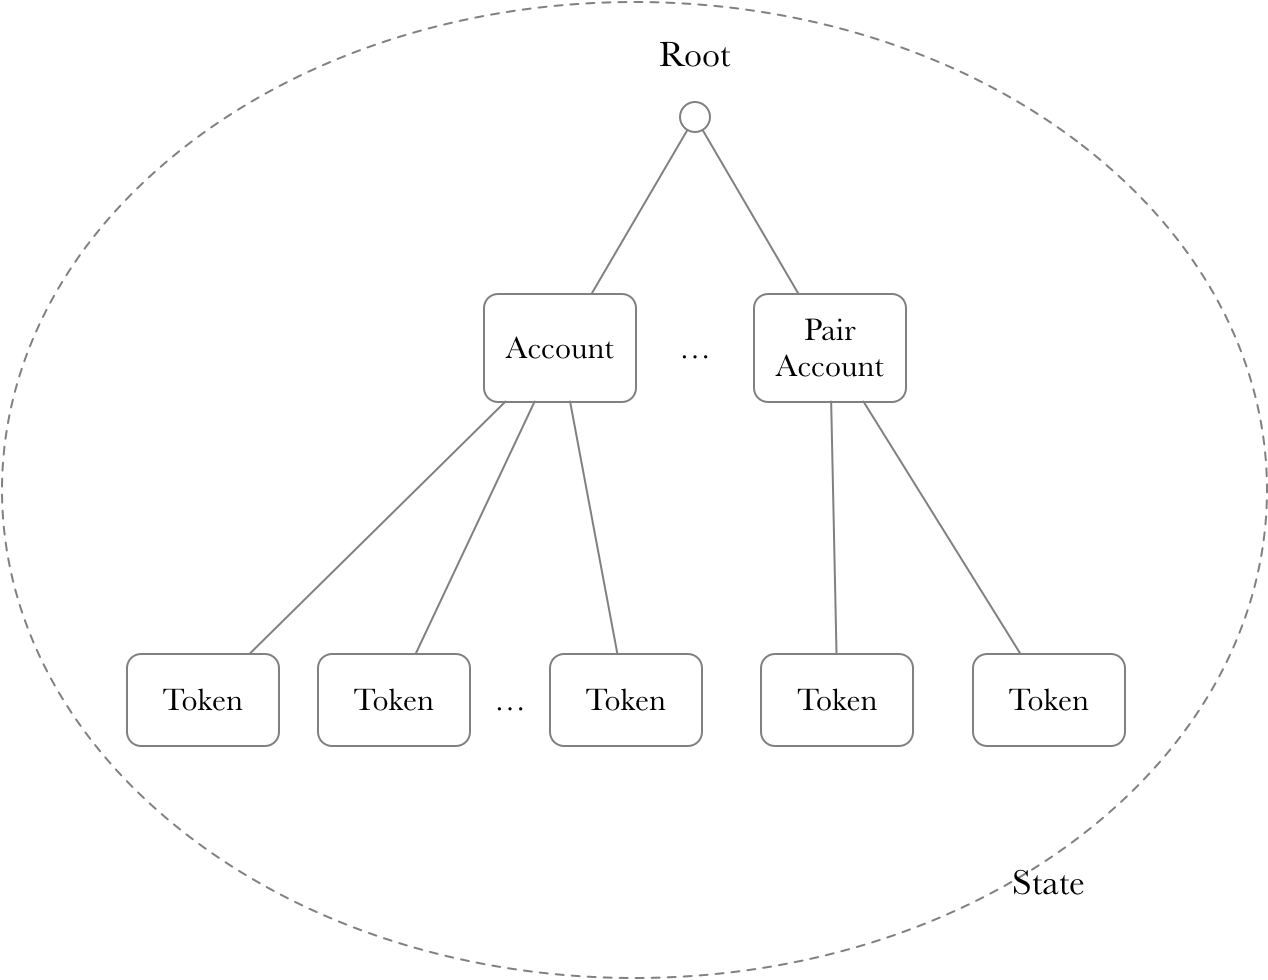
\includegraphics[width=0.9\columnwidth]{figure/state}
\caption{State}
\label{fig:state}
\end{figure}

The status tree of the ZKSwap system records the balance of all accounts in the current system. The state tree of ZKSwap is a Merkel tree with a height of 34. The child nodes of the Root are all account nodes (24 levels) in the system. There are two types of account nodes: 


\begin{itemize}
	\item Ordinary account node: to record the status of all tokens in the account. Ordinary account nodes can have any number of leaf nodes (10 levels), each leaf node represents a type of token and its amount; there can’t be repeated token types within one account.
	\item Pair account node: to record the status of the liquidity pool of a certain pair of assets ZKSwap. The Pair Account Node contains only two leaf nodes. Each leaf node represents the balance and type of one token in the liquidity pool.
\end{itemize}

The transaction process in ZKSwap is essentially the process of updating the state tree. The following section will be the introduction of all transaction types in ZKSwap and their corresponding State changes.

\subsection{Deposit}

\begin{figure}[htbp]
\centering
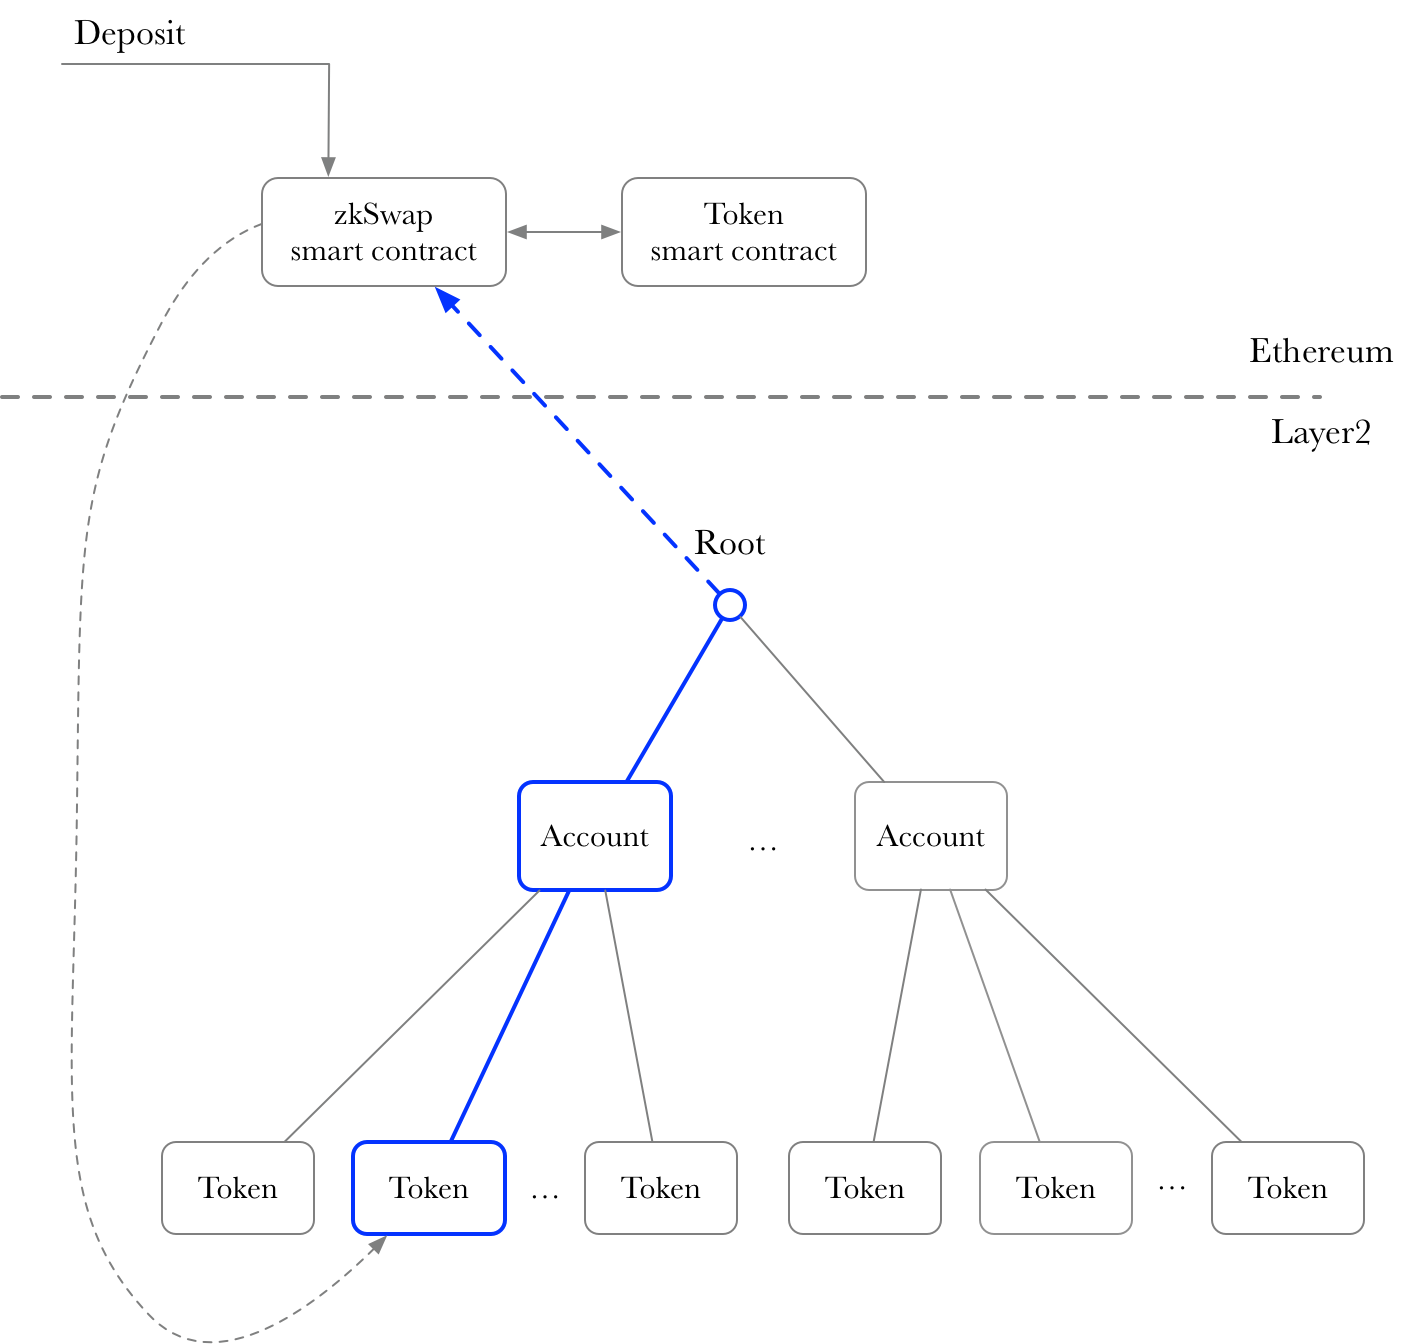
\includegraphics[width=0.9\columnwidth]{figure/deposit}
\caption{Deposit}
\label{fig:deposit}
\end{figure}

Deposit refers to the process where users deposit Ethereum and ERC20 tokens into the ZKSwap contract so that those tokens can be used on Layer 2. The Deposit process is initiated by the user on-chain. When ZKSwap Server monitors that the user transfers tokens to the ZKSwap smart contract, it will update the Status Tree according to the transaction details. First, it will find the corresponding Account to which the transaction belongs, then update the status of the corresponding Token under that Account based on the Deposited amount. If there is no leaf node corresponding to the Token under this Account, then first create the leaf node corresponding to the Token, and then update the status. When the status of the leaf node is updated, the hash of the root node will be updated accordingly.

The updated hash of the root node of the state tree, together with the SNARK proof of the Deposit transaction, will be sent to the ZKSwap contract on-chain.

\subsection{Withdraw}

\begin{figure}[htbp]
\centering
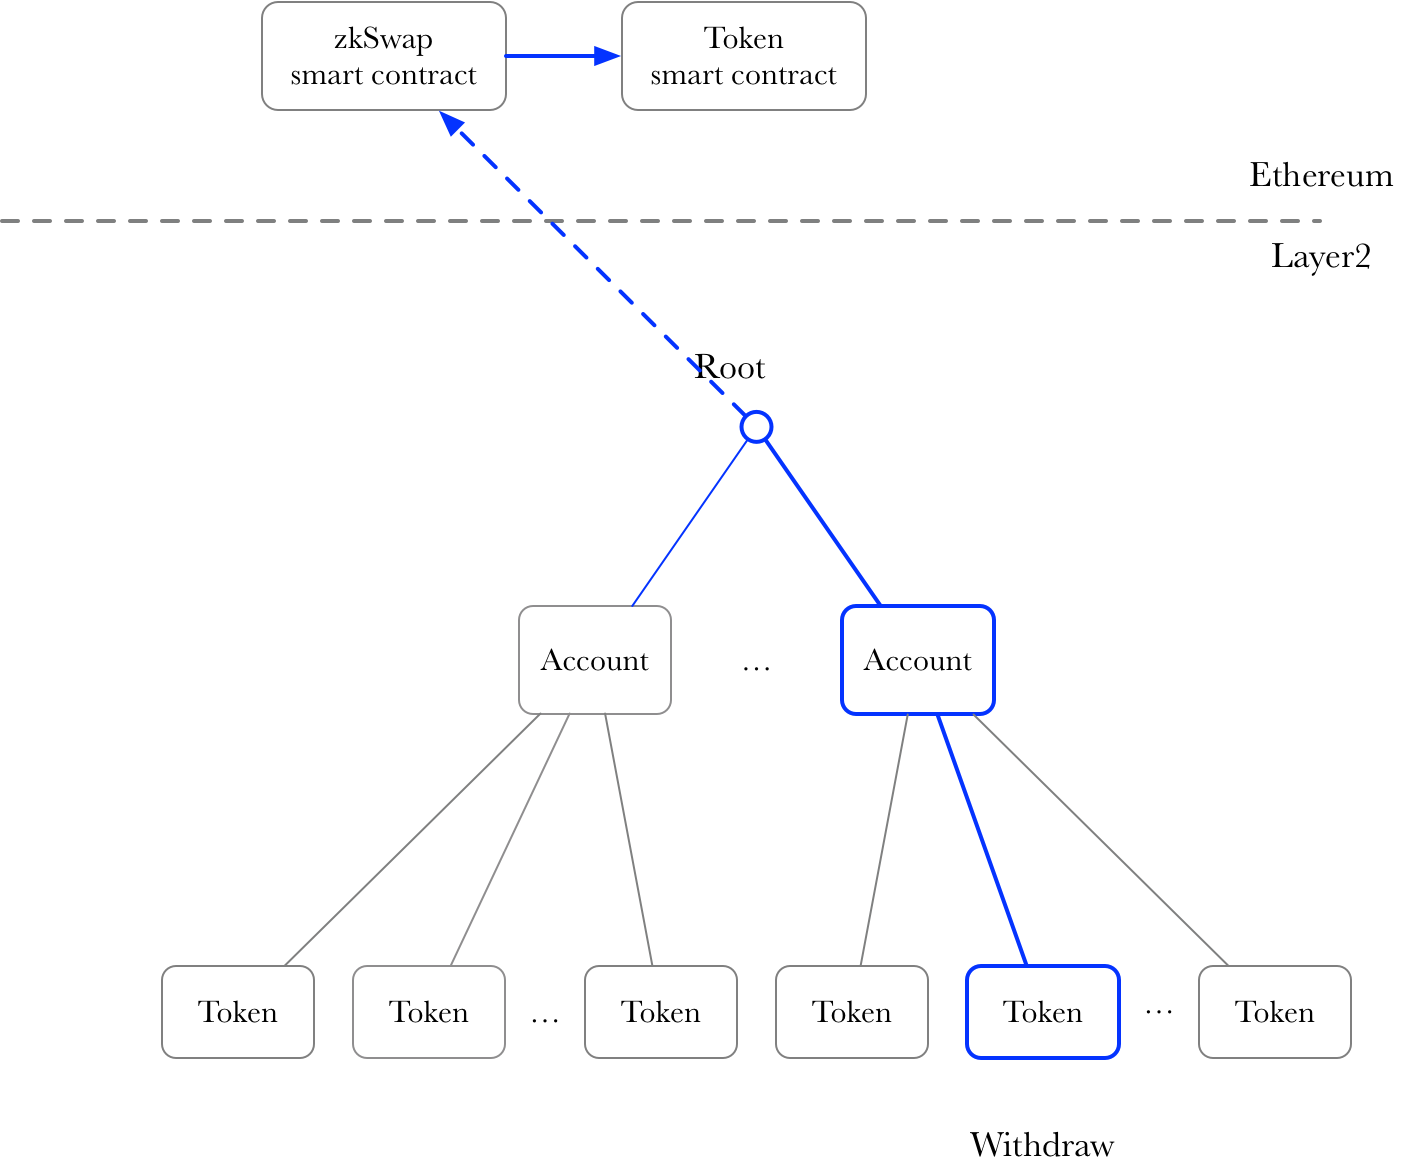
\includegraphics[width=0.9\columnwidth]{figure/withdraw}
\caption{Withdraw}
\label{fig:withdraw}
\end{figure}

Withdraw means that the user withdraws the Token from Layer 2, unlocks it from the ZKSwap contract, and sends it to the corresponding Layer 1 account. The Withdraw process is initiated by the user from Layer 2. When the ZKSwap Server receives the user’s withdrawal request, it will update the status of the corresponding Token under the corresponding account, and send the updated root node hash and the proof of the Withdraw process to the ZKSwap contract on-chain. After the smart contract verifies it as valid, the contract will unlock the corresponding Token and send it to the account on the corresponding chain.


\subsection{Transfer}

\begin{figure}[htbp]
\centering
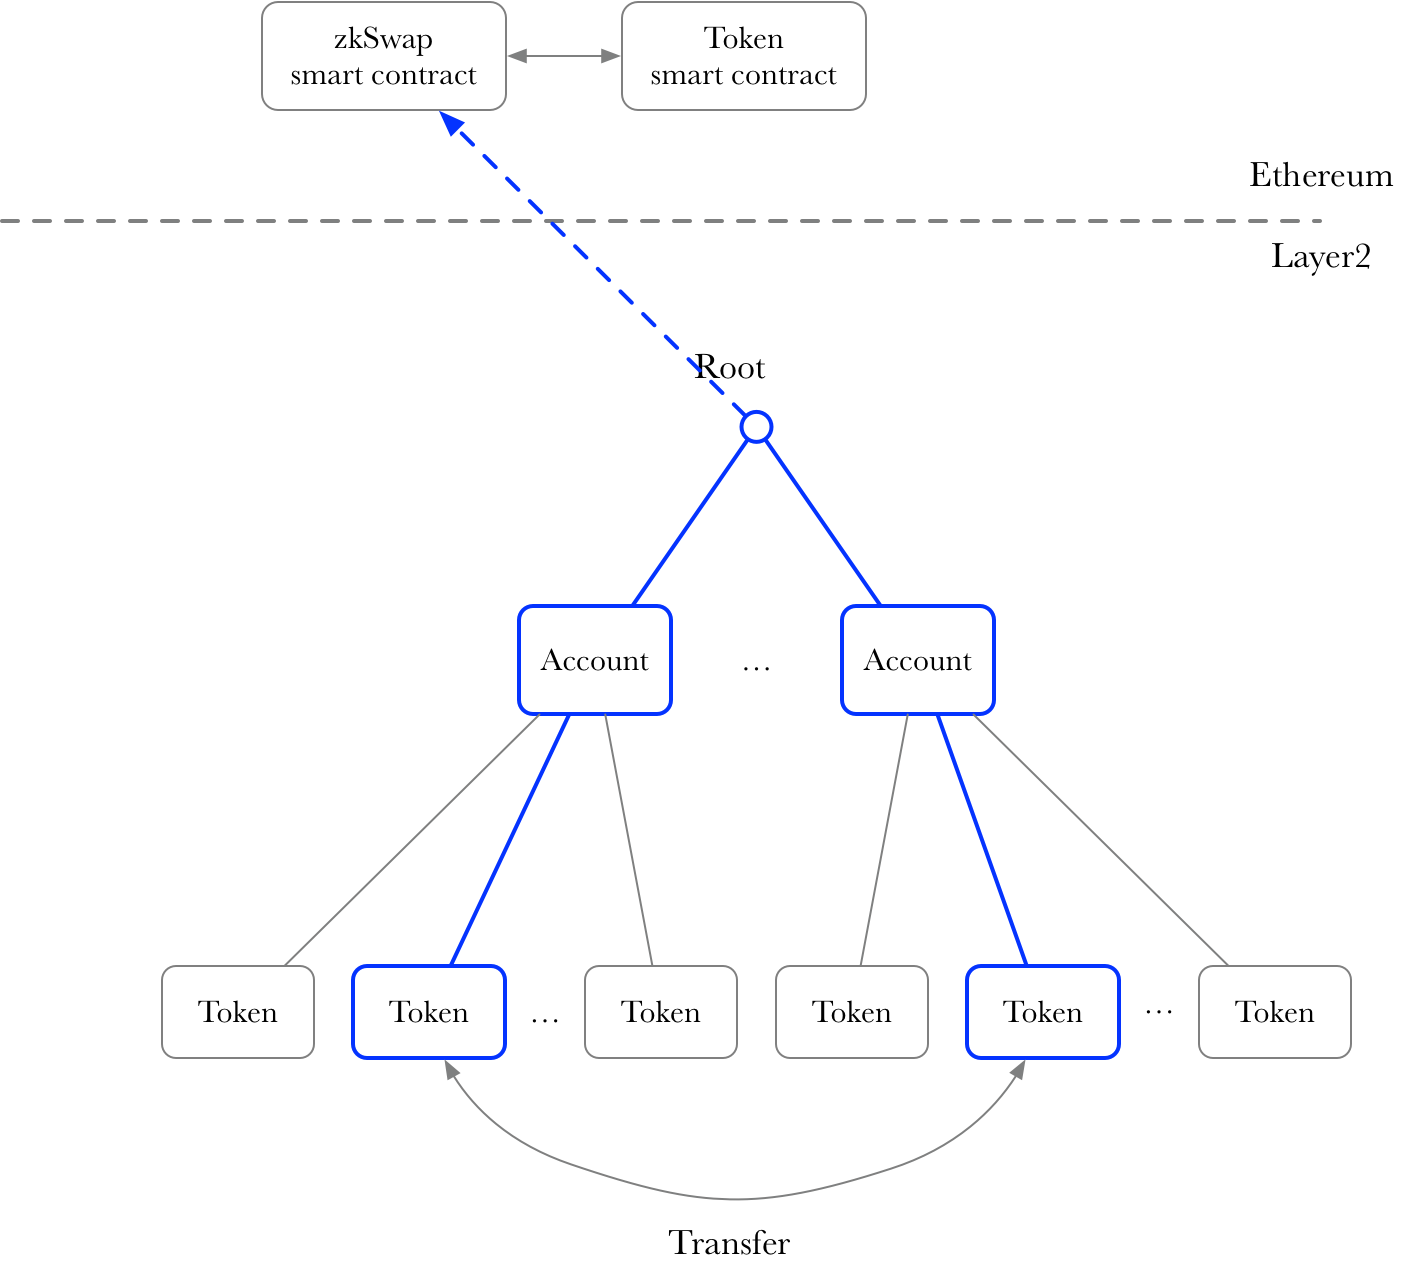
\includegraphics[width=0.9\columnwidth]{figure/transfer}
\caption{Transfer}
\label{fig:transfer}
\end{figure}

Transfer refers to the process where one user sends a certain token to another user in ZKSwap Layer 2. The Transfer process is initiated by the user on Layer 2. When the ZKSwap Server receives the Transfer request, it will find the corresponding sending and receiving accounts according to the request details.
And it will update the status of the Token under the accounts of the sender and receiver according to the sent amount. The hash of the root node of the state tree will be updated accordingly, and together with the SNARK proof corresponding to the Transfer operation, be sent to the contract on the ZKSwap smart contract on-chain. Transfer does not change the on-chain status of the token, because the token is still locked in the ZKSwap contract and has not been transferred on-chain.


\subsection{Create Liquidity}

\begin{figure}[htbp]
\centering
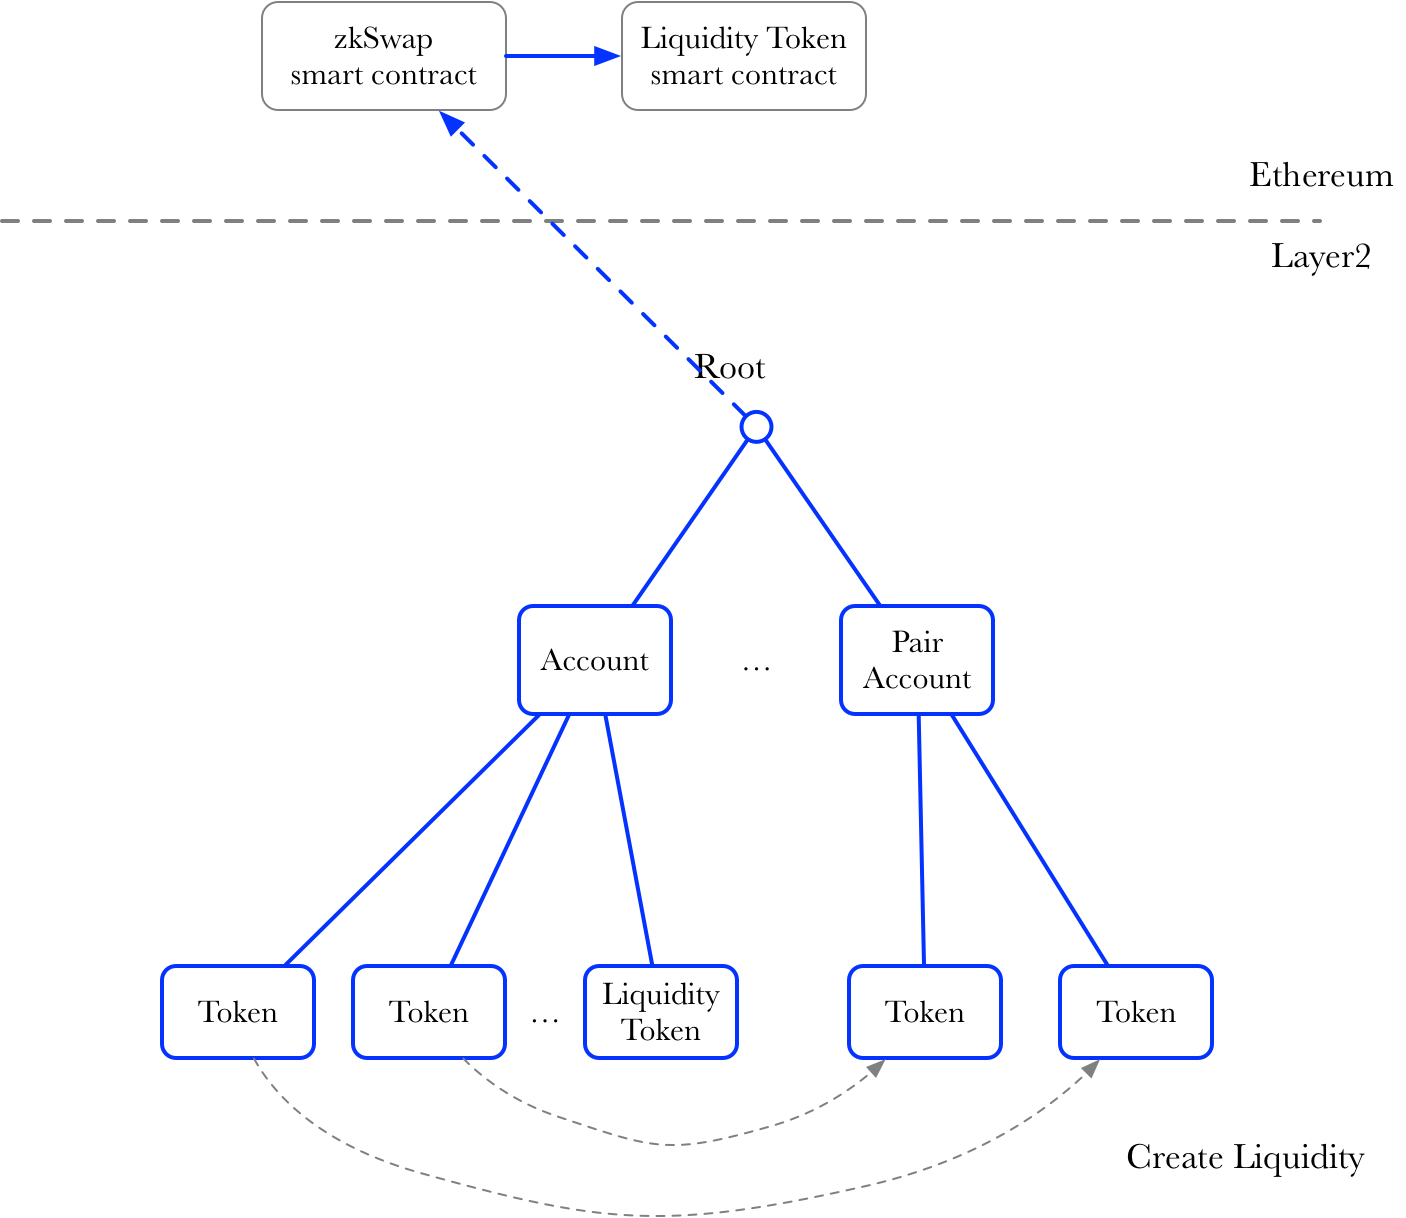
\includegraphics[width=0.9\columnwidth]{figure/create_liquidity}
\caption{Create Liquidity}
\label{fig:create_liquidity}
\end{figure}

Create liquidity refers to the process where the user creates a liquidity pool or adds liquidity to an existing pool on Layer 2. The definition remains the same as that in Uniswap. 
Create Liquidity is initiated by the user on Layer 2. When the ZKSwap Server receives the user’s request to create liquidity for a pair of assets, it first needs to find the initiator’s Account and the Pair Account of the pair of tokens (If the Pair Account does not exist, the user needs to create a Pair liquidity pool first);  then, transfer the two Tokens are calculated according to the AMM algorithm.
to the Pair Account proportionately; at the same time, the system will calculate the number of LP Tokens the user will receive, and update the corresponding LP Token status under the liquidity provider Account. After all status updates are completed, the status tree root node hash will be sent to the ZKSwap smart contract on-chain together with the proof of Create Liquidity. The initial minted LP token will need to be done by the ZKSwap Contract to deploy the corresponding LP Token contract on-chain.


\subsection{Remove Liquidity }

\begin{figure}[htbp]
\centering
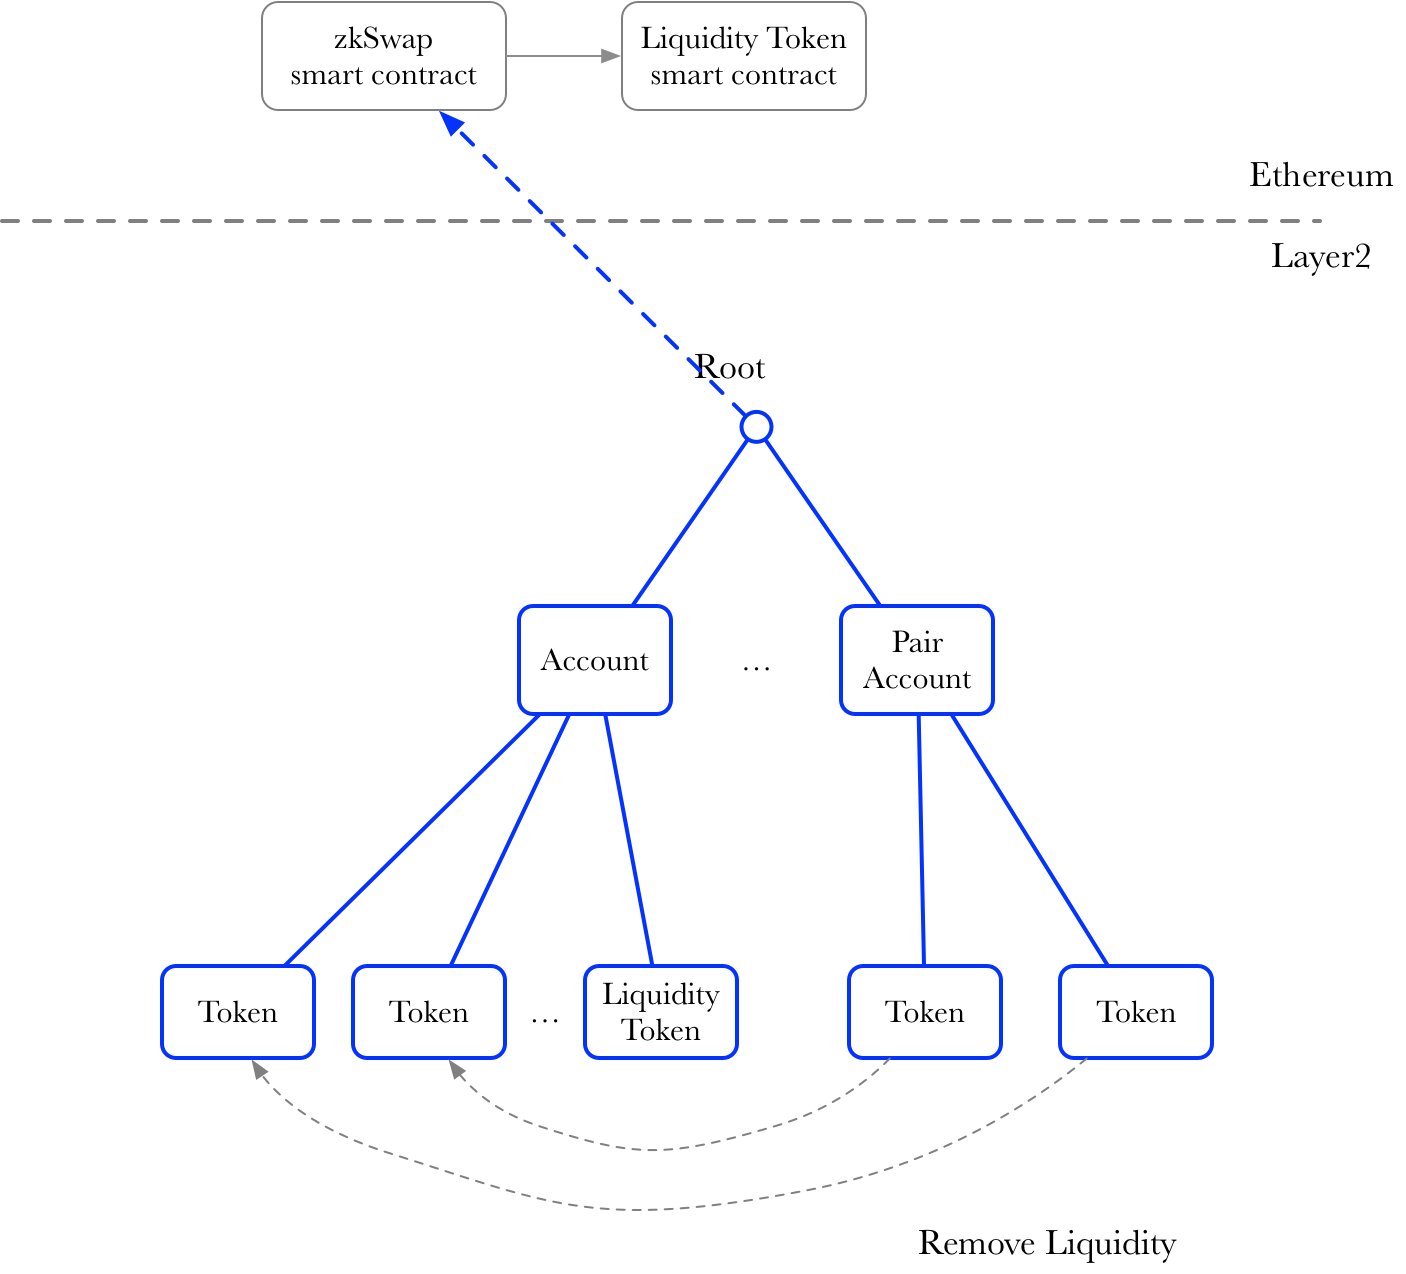
\includegraphics[width=0.9\columnwidth]{figure/remove_liquidity}
\caption{Remove Liquidity}
\label{fig:remove_liquidity}
\end{figure}

Remove Liquidity refers to the process where the user burns the LP Token from a certain Pair liquidity pool on Layer 2 and withdraws the two tokens from the pool reserve. Remove Liquidity is initiated by the user on Layer 2, when ZKSwap Server receives a user’s Remove Liquidity request, it will first find the corresponding Account and burn the corresponding amount of Liquidity Tokens; then the two Tokens under the Pair Account corresponding to Liquidity Token will be proportionately transferred to the Account which has just burned its Liquidity Tokens. After the process is completed, the state tree will be updated accordingly, and the root node hash and the proof of the corresponding Remove Liquidity operation will be sent to the ZKSwap contract on-chain.

\pagebreak


\subsection{Swap }

\begin{figure}[htbp]
\centering
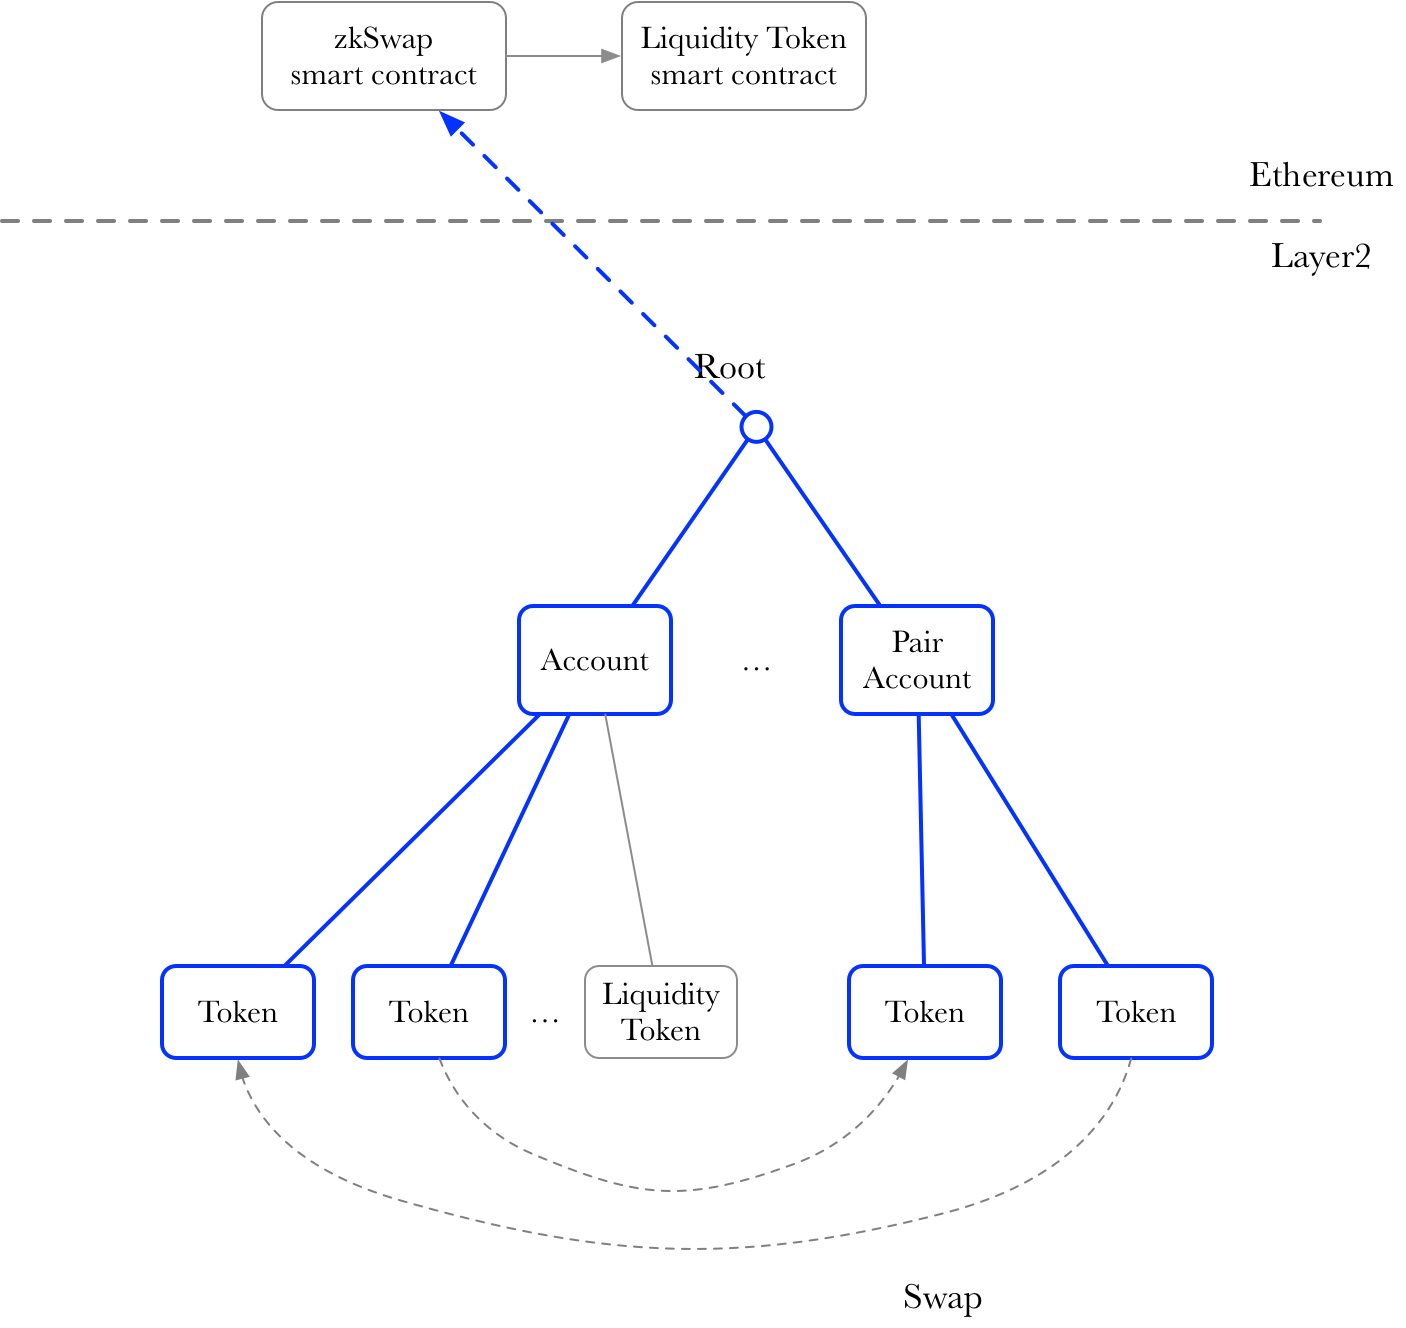
\includegraphics[width=0.9\columnwidth]{figure/swap}
\caption{Swap}
\label{fig:swap}
\end{figure}

Swap refers to the process where users complete transactions in the Layer 2 liquidity pools. Suppose the user needs to swap in the pool that contains TokenA -TokenB Pair Token. The user first sends TokenA from his account on Layer 2 to the corresponding Pair Account. Then ZKSwap will calculate the number of TokenB for the user according to the AMM algorithm and send it to the user. The state tree is updated accordingly. The ZKSwap Server will update the root node hash of the state tree. The hash and the swap proof will be sent to the ZKSwap contract on-chain. Swap transactions will not change the status of the token on-chain, because the token itself is still locked in the ZKSwap contract.


\subsection{Withdraw Liquidity}

\begin{figure}[htbp]
\centering
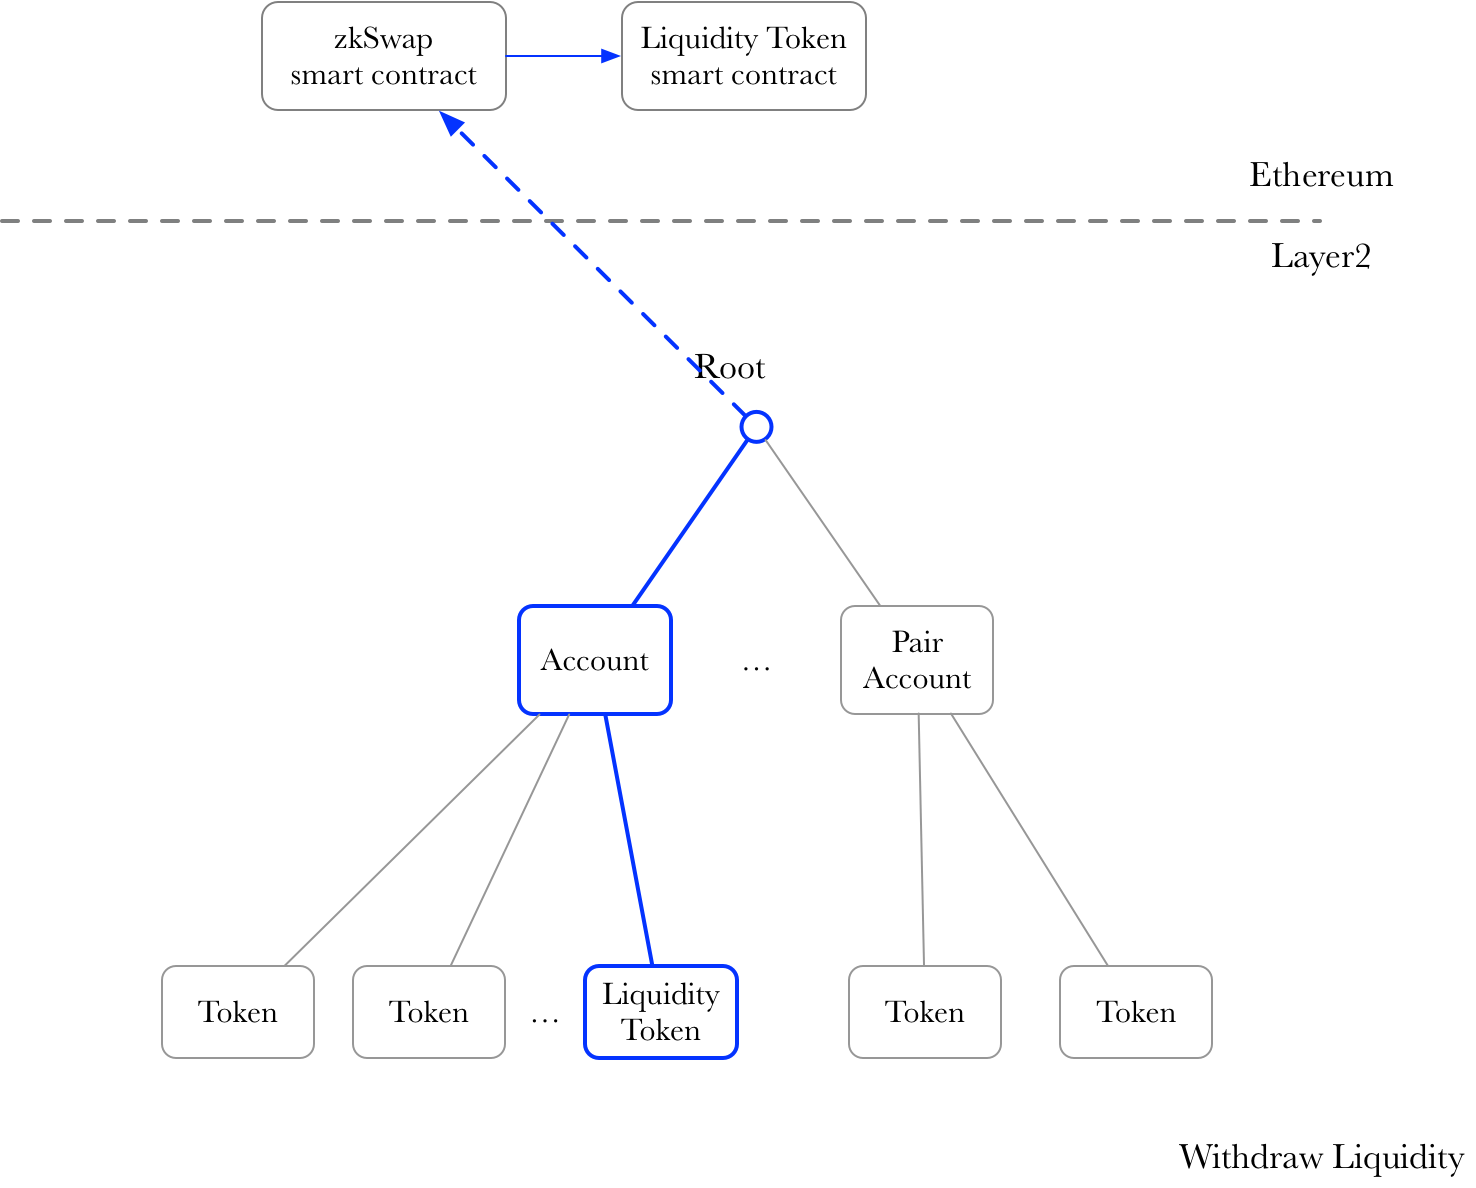
\includegraphics[width=0.9\columnwidth]{figure/withdraw_liquidity}
\caption{Withdraw Liquidity}
\label{fig:withdraw_liquidity}
\end{figure}

Withdraw Liquidity refers to the process where the user withdraws the Liquidity Token from the Layer 2 account to Layer 1. Withdraw Liquidity’s initiation process and status update on Layer 2 are exactly the same as the above-mentioned ordinary Withdraw, but it produces different results on Layer 1. After the ZKSwap contract receives the Withdraw Liquidity request, it will automatically trigger Liquidity Token minting to mint additional Liquidity Tokens onLayer 1 and send it to the designated account.


\section{Summary and Outlook}

ZKSwap uses ZK-Rollup technology to realize the complete function of Uniswap in Layer-2. It is a set of decentralized Layer-2 token AMM (Automated Market Maker) Swap protocol, with infinite scalability and high TPS. Liquidity providers and users do not need to pay high gas fees and always have real-time transactions. Users no longer need to wait for block confirmations to complete transactions on Layer 2, which dramatically reduces the threshold for using DEX and brings significant changes to all current DEX and CEX.

ZKSwap is developed with the support of L2 Lab. In the future, L2 Lab will continue to promote the development of the Layer 2 protocol layer, combining a series of Layer 2 basic protocols such as ZKSwap and Layer 2 privacy stable coins to create a complete Layer 2 DeFi ecosystem.

By creating a Layer-2 protocol standard with excellent user experience, L2 Lab is committed to promoting the paradigm shift in the blockchain industry, making Layer 1 the foundation of clearing and settlement, and Layer 2 connecting blockchain applications and Layer 3 bridges and entrances. We are committed to promoting all blockchain applications to run in a layer-3 world without any restrictions.

We will be committed to making ZKSwap the most useful product in DEX. When the time is right, we will also launch a liquid mining plan, and DAO plans to help the rise of distributed financial DeFi and lead the paradigm change of blockchain applications.



\bibliographystyle{template/splncs04}
\bibliography{zkswap.bib}

\end{document}